\documentclass[11pt,a4paper]{article}

\usepackage[T1]{fontenc}
\usepackage[utf8]{inputenc}
\usepackage[spanish,es-tabla,es-noshorthands,es-nodecimaldot]{babel}
\usepackage{lmodern}
\usepackage{microtype}
\usepackage[margin=2.5cm]{geometry}
\usepackage{amsmath,amssymb}
\usepackage{graphicx}
\usepackage{booktabs}
\usepackage{longtable}
\usepackage{array}
\usepackage{float}
\usepackage{caption}
\usepackage{subcaption}
\usepackage[dvipsnames]{xcolor}
\usepackage{enumitem}
\usepackage{listings}
\usepackage[round,authoryear]{natbib}
\usepackage[hidelinks]{hyperref}
\usepackage{adjustbox}

\graphicspath{{../../finetuning/results/figures/}}
\newcommand{\tabdir}{../../finetuning/results/tables}
\input{\tabdir/macros.tex}

\captionsetup{font=small,labelfont=bf}
\setlist{itemsep=2pt,topsep=4pt}
\lstset{basicstyle=\ttfamily\small,breaklines=true,columns=fullflexible,frame=single,framerule=0.3pt,rulecolor=\color{gray!60}}
\newcommand{\spp}[1]{\textit{#1}}
\DeclareUrlCommand\code{\urlstyle{tt}}
\makeatletter\g@addto@macro\UrlBreaks{\do\_\do-}\makeatother
\newcommand{\fittab}[1]{\adjustbox{max width=\linewidth}{\input{\tabdir/#1}}}
\newcommand{\R}{\mathbb{R}}
\DeclareMathOperator*{\argmin}{arg\,min}

\title{Ajuste fino de clasificadores bioacústicos para \textit{EcoAcoustic Sentinel}\\[4pt]
\large Datos AudioMoth del proyecto CONDESAN: fundamentos, metodología y resultados}
\author{EcoAcoustic Sentinel · Proyecto CONDESAN}
\date{4 de noviembre de 2026}

\begin{document}
\maketitle

\begin{abstract}
\noindent
Este informe recoge el análisis del estado del repositorio \textit{EcoAcoustic Sentinel} y el ajuste fino de su
componente de clasificación con las grabaciones AudioMoth y las validaciones expertas del proyecto CONDESAN
(6 grabadoras, 24 de julio a 6 de agosto de 2025, 88 especies validadas). Se trabajó sobre una copia local de solo lectura
de los datos de Google Drive. Las ventanas de 3\,s se representaron con los \emph{embeddings} de BirdNET V2.4, y se compararon
cinco familias de clasificadores bajo validación cruzada agrupada por sesión: BirdNET sin ajuste, BirdNET con su última
capa afinada (regularización L2-SP), los prototipos coseno que usa hoy la aplicación, sondas lineales y perceptrones multicapa.
Sobre \nWindows{} ventanas y \nSpecies{} especies objetivo, BirdNET obtiene una mAP de \mapBirdnet{}, la versión afinada \mapFT{}
(diferencia no significativa), la mejor sonda entrenada desde cero \mapLinear{} y los prototipos de la aplicación \mapProto.
La ventaja de BirdNET está inflada por un sesgo de verificación, porque las etiquetas son detecciones de BirdNET confirmadas por expertos.
Aun así, los resultados permiten tres mejoras concretas.
Primero, sustituir los prototipos por una cabeza entrenada mejora la mAP en \deltaLinearVsProto{} (IC 95\,\% \ciLinearVsProto).
Segundo, restringir BirdNET a las especies locales elimina el \nonlocalHalf\,\% de sus detecciones con puntuación $\geq 0{,}5$, que corresponden a especies ajenas a la región.
Tercero, los umbrales por especie se calibraron con el método de \citet{wood2024guidelines}.
Estas mejoras se integraron en la aplicación como un \emph{clasificador local CONDESAN} opcional.
El informe identifica además una sesión cuyos audios no corresponden a sus etiquetas y una revisión parcial
de las especies más abundantes, y enumera la ayuda manual necesaria para un conjunto de prueba sin sesgo.
\end{abstract}

\tableofcontents
\newpage

% ============================================================================
\section{Introducción y objetivos}
% ============================================================================
El monitoreo acústico pasivo permite registrar la actividad de aves durante semanas con grabadoras autónomas de bajo costo
como AudioMoth \citep{hill2018audiomoth,gibb2019passive}. El cuello de botella es el análisis: miles de horas de audio exigen
detectores automáticos cuya salida debe ser verificada y calibrada para cada sitio \citep{stowell2022review,wood2024guidelines}.

\textit{EcoAcoustic Sentinel} es una aplicación de escritorio que combina BirdNET \citep{kahl2021birdnet} con una biblioteca
de perfiles de especies definidos por el usuario. El equipo de CONDESAN recopiló una campaña completa de grabaciones en el
bosque seco y validó manualmente las detecciones de BirdNET. Los objetivos de este trabajo fueron:
\begin{enumerate}
  \item analizar lo avanzado en el repositorio e identificar los puntos de mejora del pipeline de clasificación;
  \item construir, a partir de los datos y validaciones de CONDESAN, un conjunto de entrenamiento y evaluación reproducible,
        sin modificar ni borrar nada de la carpeta original de Google Drive;
  \item ajustar (\emph{fine-tuning}) y comparar clasificadores con un protocolo que evite fugas de información;
  \item integrar el mejor modelo en la aplicación de forma aditiva y desactivada por defecto;
  \item documentar teoría, métodos, resultados y limitaciones, e indicar qué ayuda manual se requiere.
\end{enumerate}

% ============================================================================
\section{Análisis del estado del repositorio}
% ============================================================================
\subsection{Componentes existentes}
El repositorio contiene una aplicación de escritorio en Python 3.11 con interfaz PySide6 (\code{main.py}, \code{ui_theme.py}) y un
motor de análisis (\code{audio_analyzer.py}). Sus funciones principales son:
\begin{itemize}
  \item \textbf{Descubrimiento global con BirdNET V2.4} (\code{birdnet-analyzer} 2.4.0). Admite un filtro geográfico opcional
        (latitud/longitud) y un solapamiento configurable entre ventanas.
  \item \textbf{Biblioteca de perfiles (\emph{few-shot})}. El usuario define especies de referencia con clips de audio.
        La aplicación guarda varios vectores de \emph{embedding} por perfil y clasifica cada ventana por la máxima
        similitud coseno contra esos vectores, con un umbral global (0,75 por defecto) y suavizado temporal.
  \item \textbf{Estrategia híbrida}. Si hay coincidencias con perfiles propios, se priorizan; las detecciones de BirdNET de
        baja confianza que no solapan con ellas se marcan como \emph{anomalías} para revisión.
  \item \textbf{Herramientas auxiliares}: visor de espectrograma con eje en Hz, reducción de ruido opcional (\code{noisereduce}),
        exportación a CSV, Raven, Audacity y Kaleidoscope, y empaquetado con PyInstaller e instalador Inno Setup.
\end{itemize}

\subsection{Limitaciones detectadas}
\begin{enumerate}
  \item \textbf{Sin evaluación cuantitativa}. No existía un conjunto etiquetado ni métricas para comparar la biblioteca de perfiles con BirdNET.
  \item \textbf{Umbral único}. El umbral coseno es el mismo para todas las especies, aunque la separabilidad de cada especie en el espacio de \emph{embeddings} es muy distinta (sección~\ref{sec:resultados}).
  \item \textbf{Lista de especies global}. Sin coordenadas, BirdNET considera sus 6\,522 clases, incluidas especies de otros continentes que se confunden con congéneres locales.
  \item \textbf{Ningún uso de las validaciones de CONDESAN}. Las miles de detecciones revisadas por expertos no se aprovechaban para calibrar el sistema.
\end{enumerate}

\subsection{Aportes de este trabajo}
Se añadió el paquete \code{finetuning/} (pipeline reproducible de datos, \emph{embeddings}, entrenamiento, evaluación y figuras),
el módulo \code{local_classifier.py} con su integración opcional en la aplicación, el modelo exportado en
\code{local_models/condesan/} y este informe. Todos los cambios en archivos existentes son aditivos: con la nueva opción desactivada,
la aplicación se comporta exactamente igual que antes.

% ============================================================================
\section{Marco teórico}
% ============================================================================
\subsection{Representación tiempo-frecuencia del sonido}
Una grabación digital es una secuencia $x[n]$ muestreada a $f_s$ (48\,kHz en este estudio). Los cantos de aves son señales no
estacionarias: su contenido espectral cambia en decenas de milisegundos. La transformada de Fourier de tiempo corto (STFT) las describe localmente
\citep{oppenheim2010dsp}:
\begin{equation}
  X(m,k) = \sum_{n} x[n]\, w[n - mH]\, e^{-j 2\pi k n / N},
\end{equation}
donde $w$ es una ventana de longitud $N$ y $H$ el salto entre tramas. El espectrograma $|X(m,k)|^2$ muestra la energía en el
plano tiempo-frecuencia. La longitud de la ventana fija un compromiso: más resolución en frecuencia implica menos resolución en tiempo.
Las redes neuronales para bioacústica suelen usar espectrogramas en escala mel, $\mathrm{mel}(f) = 2595 \log_{10}(1 + f/700)$
\citep{stevens1937mel}, con compresión logarítmica de la amplitud \citep{stowell2022review}.

\subsection{BirdNET}
BirdNET \citep{kahl2021birdnet} es una red convolucional entrenada con decenas de miles de horas de grabaciones etiquetadas. La versión 2.4
usa un esqueleto de la familia EfficientNet \citep{tan2019efficientnet}. Recibe segmentos de 3\,s a 48\,kHz, calcula internamente
espectrogramas mel y produce puntuaciones para 6\,522 clases (aves y otros sonidos). Las capas finales son:
\begin{equation}
  \mathbf{e} = \mathrm{GAP}\big(f_\theta(\mathbf{x})\big) \in \R^{1024}, \qquad
  \mathbf{z} = W^\top \mathbf{e} + \mathbf{b}, \qquad
  p_c = \sigma(s \cdot z_c) = \frac{1}{1 + e^{-s z_c}},
\end{equation}
donde $f_\theta$ es el extractor convolucional, GAP el promedio global (\code{GLOBAL_AVG_POOL}), $W \in \R^{1024\times 6522}$ y
$\mathbf{b}$ los parámetros de la capa de clasificación (\code{CLASS_DENSE_LAYER}), y $s$ la \emph{sensibilidad} (1 por defecto).
El vector $\mathbf{e}$ es el \emph{embedding}: una representación compacta del contenido acústico de la ventana que puede reutilizarse
para otras tareas \citep{ghani2023embeddings}. Cada clase tiene su propia sigmoide, por lo que la salida es multietiqueta. La puntuación $p_c$
\emph{no} es una probabilidad calibrada de presencia: su relación con la precisión real depende de la especie y del sitio
\citep{wood2024guidelines}.

\subsection{Aprendizaje por transferencia y ajuste fino}
Un modelo preentrenado con muchos datos aprende representaciones útiles para tareas relacionadas \citep{yosinski2014transferable}.
Hay dos estrategias principales:
\begin{itemize}
  \item \textbf{Extracción de características (sonda).} Se congela $f_\theta$ y se entrena una cabeza nueva sobre $\mathbf{e}$,
        lineal ($\hat{\mathbf{y}} = \sigma(V^\top \mathbf{e} + \mathbf{c})$) o un perceptrón multicapa (MLP). Es barato y robusto con pocos datos
        \citep{ghani2023embeddings}.
  \item \textbf{Ajuste fino.} Se parte de los pesos preentrenados y se continúa el entrenamiento con los datos locales. Aquí se afinó
        únicamente la capa de clasificación de BirdNET restringida a las especies locales, $(W_S, \mathbf{b}_S)$, partiendo de los valores originales
        $(W_S^{0}, \mathbf{b}_S^{0})$.
\end{itemize}
Con pocos datos, el ajuste fino puede olvidar lo aprendido. La regularización L2-SP \citep{li2018l2sp} penaliza la distancia al punto de partida,
no al origen:
\begin{equation}
  \mathcal{L}(W_S, \mathbf{b}_S) = \mathcal{L}_{\text{datos}} + \lambda \,\big\| W_S - W_S^{0} \big\|_F^2 .
\end{equation}
Con $\lambda \to \infty$ se recupera BirdNET original; con $\lambda = 0$, un ajuste libre que puede sobreajustarse.

\subsection{Clasificación \emph{few-shot} con prototipos}
Las redes prototípicas \citep{snell2017prototypical} representan cada clase $c$ con el centroide $\boldsymbol{\mu}_c$ de los \emph{embeddings}
de sus ejemplos y clasifican por proximidad. La biblioteca de perfiles de la aplicación es una variante con similitud coseno y varios prototipos
por clase:
\begin{equation}
  s_c(\mathbf{e}) = \max_{j} \frac{\mathbf{e}^\top \boldsymbol{\mu}_{cj}}{\|\mathbf{e}\|\,\|\boldsymbol{\mu}_{cj}\|},
\end{equation}
donde los $\boldsymbol{\mu}_{cj}$ son hasta cinco centros de $k$-medias sobre los ejemplos normalizados. No requiere entrenamiento, pero ignora los
ejemplos negativos. Por eso no aprende qué dimensiones del \emph{embedding} distinguen una especie de las demás ni del ruido de fondo.

\subsection{Pérdida multietiqueta y desequilibrio}
Cada ventana puede contener varias especies o ninguna. Se usa entropía cruzada binaria (BCE) por especie con un peso para los positivos:
\begin{equation}
  \mathcal{L}_{\text{datos}} = -\frac{1}{NC}\sum_{i=1}^{N}\sum_{c=1}^{C} \Big[ w_c\, y_{ic} \log p_{ic} + (1 - y_{ic}) \log (1 - p_{ic}) \Big],
  \qquad w_c = \sqrt{\operatorname{clip}\!\big(N^-_c / N^+_c,\, 1,\, 20\big)} .
\end{equation}
El peso $w_c$ compensa que los positivos sean una pequeña fracción de las ventanas; la raíz cuadrada y el tope evitan sobrecorregir.
La optimización usa AdamW \citep{kingma2015adam,loshchilov2019adamw}, \emph{dropout}, parada temprana sobre un conjunto de validación interno
y, opcionalmente, \emph{mixup} \citep{zhang2018mixup}: $\tilde{\mathbf{e}} = \beta \mathbf{e}_i + (1-\beta)\mathbf{e}_j$,
$\tilde{\mathbf{y}} = \beta \mathbf{y}_i + (1-\beta)\mathbf{y}_j$, con $\beta \sim \mathrm{Beta}(\alpha,\alpha)$.

\subsection{Métricas de evaluación}
Para una especie y un umbral $t$, la precisión es $P(t) = \mathrm{VP}/(\mathrm{VP}+\mathrm{FP})$, la exhaustividad (\emph{recall})
$R(t) = \mathrm{VP}/(\mathrm{VP}+\mathrm{FN})$ y $F_1 = 2PR/(P+R)$. Al recorrer $t$ se obtiene la curva precisión-exhaustividad.
Su área se resume con la \textbf{precisión promedio}:
\begin{equation}
  \mathrm{AP} = \sum_{n} (R_n - R_{n-1})\, P_n ,
\end{equation}
con los puntos ordenados por puntuación decreciente. La AP es más informativa que el área bajo la curva ROC cuando los positivos son raros
\citep{davis2006prroc,saito2015prc}. Como métrica global se usa la \textbf{mAP macro}, la media de la AP por especie, que da el mismo peso a especies
raras y abundantes. Se informan también el AUC-ROC, el $F_1$ en el umbral óptimo y \textbf{Rec@P90}, la máxima exhaustividad con precisión
$\geq 0{,}9$, que es la operación habitual en monitoreo.

\subsection{Calibración de umbrales}
\citet{wood2024guidelines} recomiendan convertir las puntuaciones de BirdNET en probabilidades de detección correcta por especie con
regresión logística sobre detecciones verificadas, en la línea de la calibración de \citet{platt1999probabilistic}:
\begin{equation}
  \Pr(\text{correcta} \mid p) = \sigma\big(\beta_0 + \beta_1 \operatorname{logit}(p)\big),
  \qquad t_{\pi} = \min\{\, p : \Pr(\text{correcta}\mid p) \geq \pi \,\}.
\end{equation}
El umbral $t_{\pi}$ garantiza, bajo el modelo, una precisión mínima $\pi$ (aquí $\pi = 0{,}90$).

\subsection{Validación sin fugas de información}
Las ventanas de una misma grabación, o de la misma grabadora en la misma mañana, comparten ruido de fondo, individuos y condiciones.
Si se reparten al azar entre entrenamiento y prueba, el modelo reconoce el contexto y no la especie, y las métricas resultan optimistas
\citep{kaufman2012leakage,roberts2017cv}. Por eso se usaron:
\begin{itemize}
  \item \textbf{Validación cruzada agrupada}: la unidad de partición es la \emph{sesión} (grabadora $\times$ día $\times$ periodo), nunca la ventana.
  \item \textbf{Grabadora fuera} (\emph{leave-one-device-out}, LODO): se entrena sin una grabadora completa y se evalúa en ella, lo que simula un sitio nuevo.
  \item \textbf{Bootstrap por conglomerados} \citep{efron1993bootstrap}: para comparar dos métodos se remuestrean sesiones con reemplazo y se
        recalcula $\Delta\mathrm{mAP}$; los percentiles 2,5 y 97,5 dan el intervalo de confianza del 95\,\%.
\end{itemize}

\subsection{Sesgo de verificación}\label{sec:sesgo}
Cuando las etiquetas de referencia se obtienen verificando solo las salidas de un detector, la evaluación queda sesgada a su favor:
los positivos que el detector no propuso nunca se etiquetan y cuentan como negativos. En diagnóstico clínico este fenómeno se conoce
como \emph{sesgo de verificación} \citep{begg1983verification}. Es central para interpretar los resultados (sección~\ref{sec:discusion}).

% ============================================================================
\section{Datos}
% ============================================================================
\subsection{Campaña AudioMoth -- CONDESAN}
La carpeta compartida \emph{AudioMoth -- CONDESAN} contiene grabaciones de seis grabadoras (AM001, AM002, AM003, AM005, AM007 y AM008),
del 24 de julio al 6 de agosto de 2025. Están organizadas por grabadora, fecha y periodo (amanecer, \emph{Sunrise}; atardecer, \emph{Sunset}).
Cada archivo WAV dura 55\,s a 48\,kHz. La subcarpeta \code{Resultados} incluye \code{TablaFinal.xlsx} con 15\,992 detecciones de BirdNET revisadas
por el equipo: 15\,913 válidas (99,5\,\%) y 79 rechazadas. Abarcan 88 especies, 4\,041 grabaciones y 89 sesiones, con nombre científico y común,
gremio trófico, categoría UICN, tiempos, frecuencias y la confianza de BirdNET.

\subsection{Copia local de trabajo}
El entorno de ejecución no podía descargar directamente desde Google Drive. Por eso se construyó una copia local de solo lectura
(\code{data_cache/drive_copy}, excluida de git) mediante el conector de Drive, con este procedimiento:
\begin{enumerate}
  \item Se seleccionó un subconjunto de grabaciones con un algoritmo voraz (\code{finetuning/select_subset.py}). Prioriza cubrir una cuota de
        positivos por especie, la diversidad de sesiones y la presencia de negativos explícitos.
  \item Cada archivo se localizó por grabadora, fecha, periodo y marca de tiempo. Hubo que tolerar variantes de nombre de carpeta (\code{Audios_*}, \code{Audio_sunrise})
        y prefijos de número de serie en los nombres de archivo.
  \item Cada descarga se decodificó y se verificó como WAV válido antes de guardarla con la misma jerarquía que en Drive (\code{finetuning/drive_mirror.py}).
\end{enumerate}
Se copiaron 257 grabaciones (1,3\,GB) más \code{TablaFinal.xlsx}. \textbf{No se modificó, movió ni borró nada en Google Drive}: todas las operaciones fueron de lectura.
Nueve grabaciones de AM003 referenciadas en TablaFinal no existen en la carpeta de Drive (sección~\ref{sec:ayuda}).

\subsection{Construcción del conjunto de ventanas}
Cada grabación se dividió en ventanas consecutivas de 3\,s, como hace BirdNET. Para cada ventana y especie objetivo
(33 especies con al menos 15 detecciones validadas) se definió:
\begin{itemize}
  \item \textbf{positivo}, si hay una detección validada de la especie en esa ventana;
  \item \textbf{negativo explícito}, si el experto rechazó la detección (\code{Valid}=0);
  \item \textbf{incierto}, si BirdNET (recalculado) da $\geq 0{,}5$ a la especie pero la detección no figura en TablaFinal;
  \item \textbf{negativo implícito}, en el resto de casos, incluidas las ventanas sin ninguna especie (\emph{fondo}).
\end{itemize}
La tabla~\ref{tab:dataset} resume el conjunto y la figura~\ref{fig:counts} compara los positivos disponibles por especie.

\begin{table}[H]
  \centering\small
  \caption{Resumen del conjunto de datos analizado.}\label{tab:dataset}
  \fittab{tab_dataset.tex}
\end{table}

\begin{figure}[H]
  \centering
  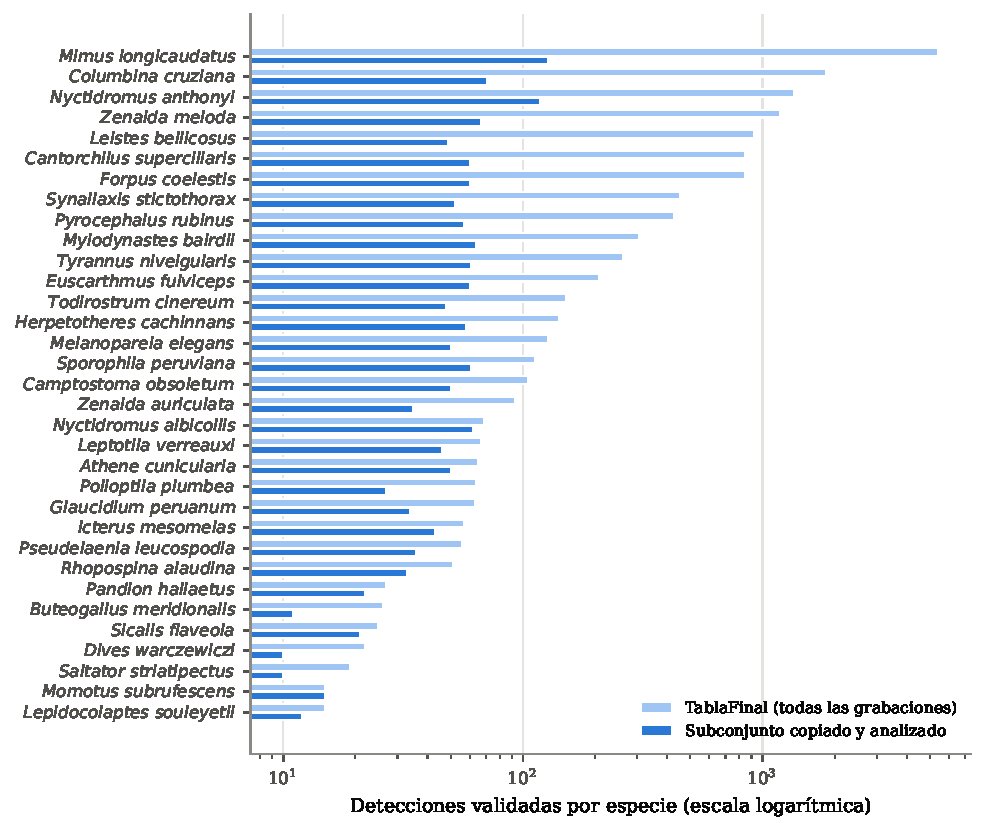
\includegraphics[width=0.82\linewidth]{fig_species_counts.pdf}
  \caption{Detecciones validadas por especie objetivo en TablaFinal (todas las grabaciones) y en el subconjunto copiado. La selección
  aplana la distribución: limita las especies muy abundantes y conserva todos los ejemplos de las raras.}\label{fig:counts}
\end{figure}

\subsection{Control de calidad: una sesión desalineada}\label{sec:qc}
Para comprobar que audio y etiquetas corresponden, se recalculó la confianza de BirdNET en cada detección de TablaFinal y se comparó con la registrada por
el equipo. Con la misma versión del modelo y la misma segmentación, ambas deben coincidir. En conjunto coincide el \qcAgreement\,\% de las filas
(diferencia $\leq 0{,}02$), pero la sesión \code{AM001_20250804_Sunrise} solo alcanza el \qcExcludedAgreement\,\%. Sus audios no corresponden a las detecciones
anotadas: es probable que la carpeta contenga grabaciones de otro día o grabadora, o que los archivos se renombraran. La sesión se excluyó
automáticamente (umbral de concordancia del 50\,\%). En las sesiones restantes la concordancia es del \qcAgreementKept\,\%, lo que confirma que
el pipeline reproduce exactamente las puntuaciones del equipo.

% ============================================================================
\section{Metodología}
% ============================================================================
\subsection{Extracción de \emph{embeddings}}
Se usó BirdNET V2.4 (FP32, TFLite) con la misma ruta de código que la aplicación (\code{birdnet_analyzer}): lectura con
\code{librosa} a 48\,kHz, segmentos de 3\,s sin solapamiento y, por segmento, una sola inferencia de la que se leen tanto los logits como
el tensor previo a la capa densa (el \emph{embedding} de 1\,024 dimensiones). Se verificó numéricamente que este tensor coincide con el que
devuelve la función oficial de \emph{embeddings}. También se extrajeron los pesos $W$ y $\mathbf{b}$ de \code{CLASS_DENSE_LAYER}, que permiten
reproducir los logits de BirdNET a partir del \emph{embedding}.

\subsection{Métodos comparados}
\begin{description}[leftmargin=1em]
  \item[BirdNET sin ajuste.] Puntuación original de la clase correspondiente (con equivalencias taxonómicas cuando TablaFinal usa un nombre más
        reciente, p.\,ej.\ \spp{Hesperoburhinus superciliaris} $\to$ \spp{Burhinus superciliaris}).
  \item[BirdNET afinado.] Capa densa de BirdNET restringida a las 33 especies, inicializada con los pesos originales y entrenada con BCE más L2-SP,
        con $\lambda \in \{0{,}3;\ 0{,}03;\ 0{,}003\}$, AdamW con tasa de aprendizaje $3\cdot 10^{-4}$ y parada temprana. La época 0 (BirdNET original)
        también es candidata.
  \item[Prototipos coseno.] Réplica del método de perfiles de la aplicación: hasta cinco prototipos por especie con $k$-medias y máxima similitud coseno.
  \item[Sonda lineal.] Regresión logística multietiqueta sobre el \emph{embedding}, con o sin normalización L2 de la entrada.
  \item[MLP.] Una capa oculta de 256 unidades (ReLU, \emph{dropout} 0,3), con y sin normalización L2 y \emph{mixup} ($\alpha = 0{,}4$).
\end{description}
Las cabezas entrenadas desde cero se implementaron en NumPy, con el gradiente verificado numéricamente. No dependen de PyTorch ni de TensorFlow.

\subsection{Protocolo de evaluación}
\begin{itemize}
  \item \textbf{Validación cruzada de 5 pliegues agrupada por sesión}, con pliegues equilibrados en número de ventanas. En cada pliegue, el 15\,\% de
        las sesiones de entrenamiento se reserva para la parada temprana. Así se obtienen predicciones fuera de muestra para todas las ventanas.
  \item \textbf{Tres regímenes de evaluación}:
    \emph{estricto}, con todas las ventanas y los pares sin validar como negativos;
    \emph{enmascarado}, que excluye de la evaluación los pares inciertos (BirdNET $\geq 0{,}5$ sin validar);
    y \emph{candidatos}, que evalúa solo las ventanas donde BirdNET da $\geq 0{,}1$ a la especie, como ocurriría si la cabeza
    reordenara las propuestas de BirdNET.
  \item \textbf{Bootstrap pareado} de 500 réplicas sobre sesiones para las diferencias de mAP.
  \item \textbf{LODO}: seis particiones, cada una sin una grabadora.
  \item \textbf{Curva de aprendizaje}: el entrenamiento se repite con como máximo $k \in \{3, 5, 10, 20, 40\}$ positivos por especie.
        Los positivos sobrantes se ignoran en la pérdida y la evaluación se hace sobre todas las ventanas.
\end{itemize}

\subsection{Exportación del modelo local}
El método con mayor mAP estricta se exporta a \code{local_models/condesan/condesan_local.json}. El archivo incluye la lista de especies con nombres
en español e inglés, la etiqueta de BirdNET, el umbral por especie y metadatos de evaluación. Si el método elegido es BirdNET sin ajuste, no se
guardan pesos: la aplicación los lee del modelo BirdNET ya instalado, de modo que el repositorio no redistribuye pesos de BirdNET (licencia
CC BY-NC-SA 4.0). Los umbrales se calibran según la sección~\ref{sec:umbrales}.

% ============================================================================
\section{Resultados}\label{sec:resultados}
% ============================================================================
\subsection{Comparación global de métodos}
La tabla~\ref{tab:methods} y la figura~\ref{fig:summary} resumen la validación cruzada. BirdNET sin ajuste obtiene la mayor mAP en los tres
regímenes (\mapBirdnet{} estricto, \mapBirdnetMasked{} enmascarado). El ajuste fino con L2-SP queda muy cerca (\mapFT), y su rendimiento empeora
al relajar la regularización. Entre las cabezas entrenadas desde cero, la sonda lineal con normalización L2 es la mejor (\mapLinear). El MLP no
la supera (\mapMLP), señal de que con estos datos la no linealidad adicional no compensa su varianza. Los prototipos coseno de la aplicación
son el método más débil (\mapProto).

\begin{table}[H]
  \centering\small
  \caption{Métricas macro (media sobre 33 especies) en validación cruzada agrupada por sesión. Rec@P90: exhaustividad máxima con precisión
  $\geq 0{,}9$. En negrita, el mejor valor de cada columna destacada.}\label{tab:methods}
  \fittab{tab_methods.tex}
\end{table}

\begin{figure}[H]
  \centering
  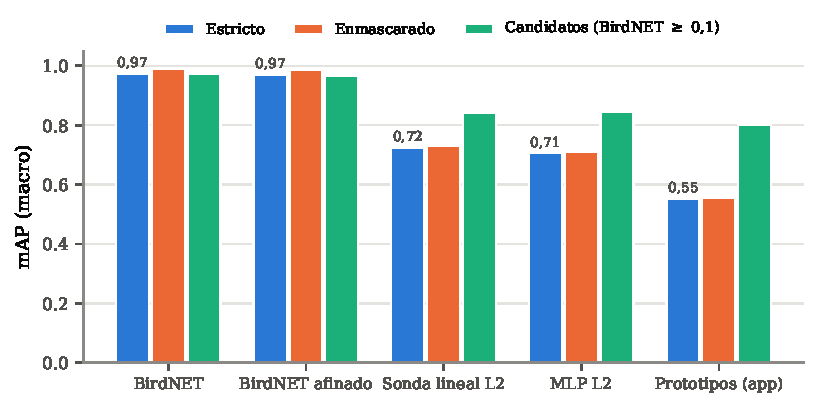
\includegraphics[width=0.9\linewidth]{fig_method_summary.pdf}
  \caption{mAP macro por método y régimen de evaluación. El régimen de candidatos acerca las cabezas entrenadas a BirdNET, pero no lo alcanzan.}\label{fig:summary}
\end{figure}

La tabla~\ref{tab:bootstrap} cuantifica la incertidumbre. La diferencia entre BirdNET afinado y BirdNET es pequeña y su intervalo incluye el
cero (\deltaFTvsBirdnet, IC \ciFTvsBirdnet). En cambio, la sonda lineal supera a los prototipos con un margen claro (\deltaLinearVsProto, IC \ciLinearVsProto).

\begin{table}[H]
  \centering\small
  \caption{Diferencias de mAP (régimen estricto) con intervalos de confianza del 95\,\% por bootstrap pareado de sesiones (500 réplicas).}\label{tab:bootstrap}
  \fittab{tab_bootstrap.tex}
\end{table}

\subsection{Resultados por especie}
La figura~\ref{fig:apspecies} muestra la AP de cada especie (la tabla completa está en el apéndice~\ref{app:species}). Las diferencias entre
métodos son mayores en especies con pocos ejemplos o cantos variables. En \spp{Glaucidium peruanum} (AP 0,02 con prototipos frente a 0,95 con
la sonda lineal), \spp{Herpetotheres cachinnans} (0,36 frente a 0,94) y \spp{Buteogallus meridionalis} (0,02 frente a 0,44), la sonda corrige total
o parcialmente el fallo de los prototipos. En \spp{Nyctidromus albicollis} y \spp{Momotus subrufescens} fallan ambos: sus positivos se
concentran en muy pocas sesiones, de modo que en algunos pliegues no hay ejemplos de entrenamiento, y solo BirdNET, que no depende de estos datos, las detecta. Las dos especies donde BirdNET obtiene la AP más baja, \spp{Mimus longicaudatus} y \spp{Leptotila verreauxi}, son las de revisión parcial
(sección~\ref{sec:umbrales}): su AP baja refleja etiquetas incompletas, no errores del modelo.

\begin{figure}[H]
  \centering
  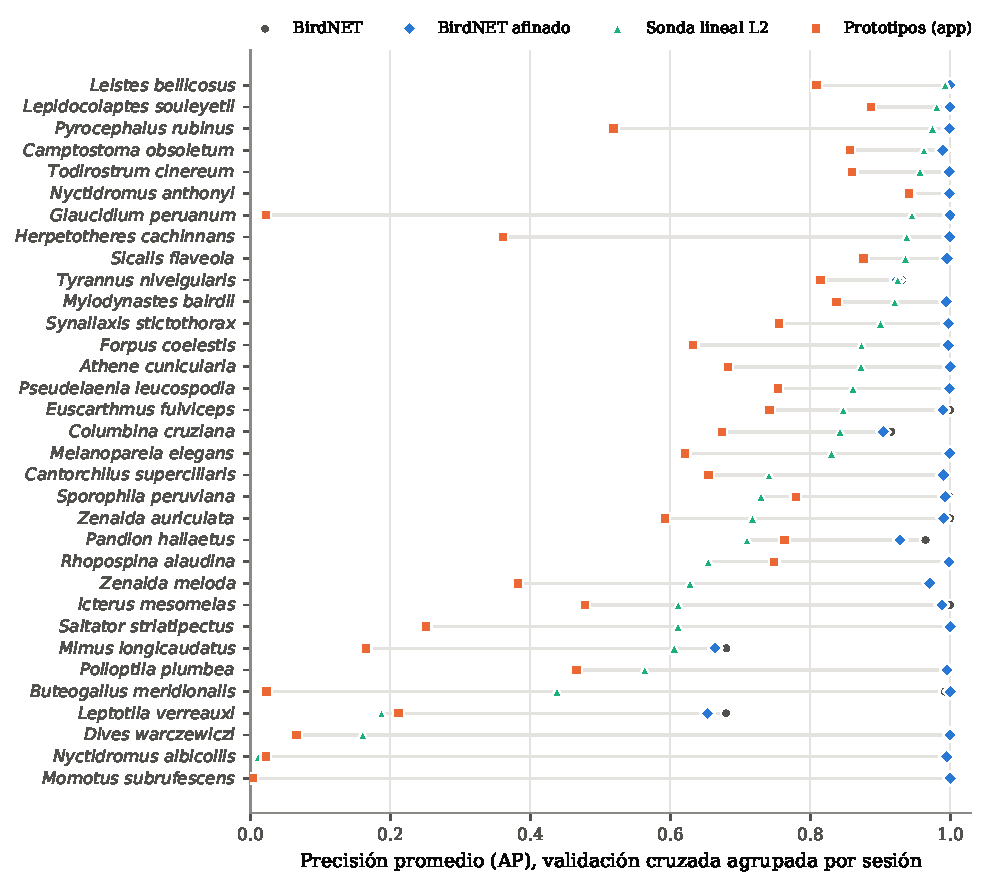
\includegraphics[width=0.86\linewidth]{fig_ap_by_species.pdf}
  \caption{Precisión promedio por especie (validación cruzada agrupada por sesión, régimen estricto), ordenada por la AP de la sonda lineal.}\label{fig:apspecies}
\end{figure}

\begin{figure}[H]
  \centering
  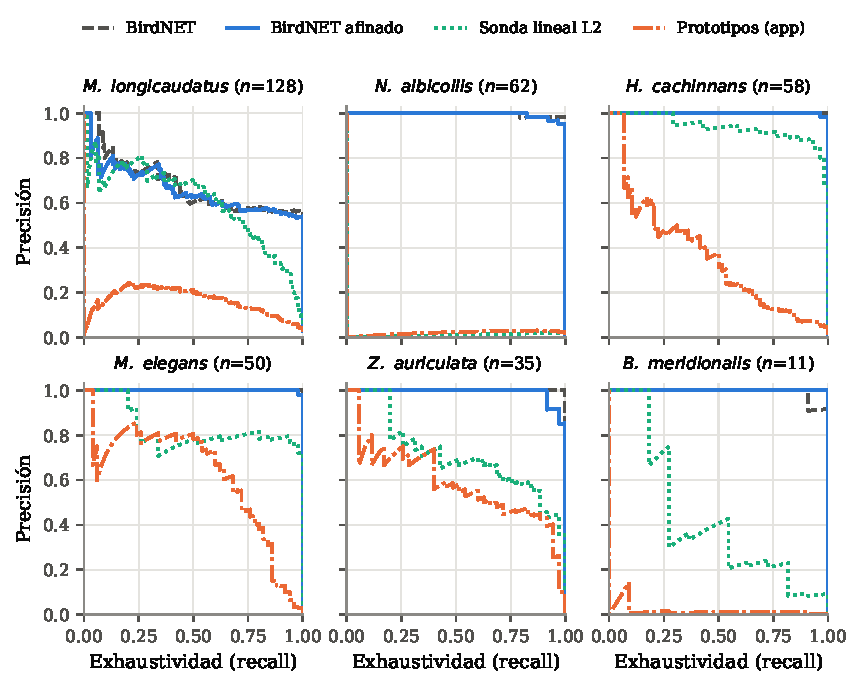
\includegraphics[width=0.95\linewidth]{fig_pr_curves.pdf}
  \caption{Curvas precisión-exhaustividad para seis especies de distinta abundancia. En \spp{M.\ longicaudatus}, la precisión de BirdNET se
  estanca en torno a 0,56 porque muchas de sus detecciones nunca fueron revisadas.}\label{fig:pr}
\end{figure}

\begin{figure}[H]
  \centering
  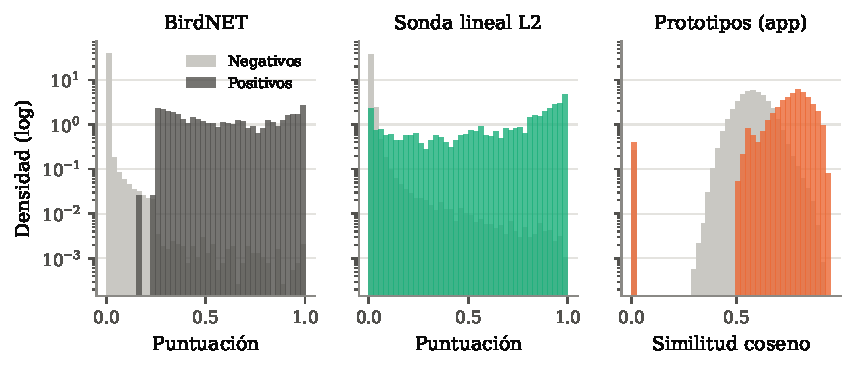
\includegraphics[width=0.95\linewidth]{fig_score_distributions.pdf}
  \caption{Distribución de puntuaciones fuera de muestra para positivos y negativos. En BirdNET los positivos empiezan bruscamente en
  $\approx 0{,}25$: es la huella del umbral con que se generaron las detecciones revisadas (sesgo de verificación). Las ventanas positivas con similitud
  0 en prototipos corresponden a pliegues sin ejemplos de entrenamiento de esa especie.}\label{fig:scores}
\end{figure}

\subsection{Generalización a grabadoras no vistas}
En LODO (tabla~\ref{tab:lodo}, figura~\ref{fig:lodo}), BirdNET mantiene una mAP media de \lodoBirdnet{}. La sonda lineal (\lodoLinear) vuelve a superar
a los prototipos (\lodoProto) en cinco de las seis grabadoras. El ajuste fino coincide con BirdNET hasta la tercera cifra decimal: la parada temprana lo mantiene en los pesos
originales o muy cerca de ellos. Las cifras de AM008 se basan en una sola especie y deben leerse con cautela.

\begin{table}[H]
  \centering\small
  \caption{mAP por grabadora retenida (\emph{leave-one-device-out}).}\label{tab:lodo}
  \fittab{tab_lodo.tex}
\end{table}

\begin{figure}[H]
  \centering
  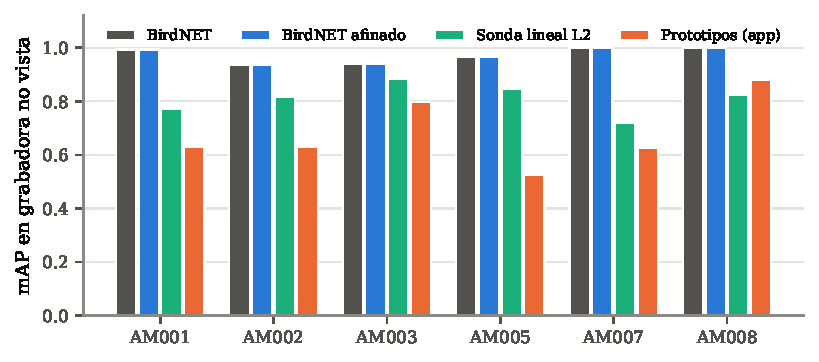
\includegraphics[width=0.9\linewidth]{fig_lodo.pdf}
  \caption{mAP en cada grabadora no vista durante el entrenamiento.}\label{fig:lodo}
\end{figure}

\subsection{Curva de aprendizaje}
La figura~\ref{fig:lc} muestra cuánto depende cada método del número de ejemplos. Con 3 positivos por especie, que es el caso típico de un perfil
creado a mano en la aplicación, prototipos y sonda lineal rinden parecido (0,40 y 0,44). A partir de 10 ejemplos la sonda se separa claramente
(0,62 frente a 0,54 con 10, y 0,71 frente a 0,55 con 40). Los prototipos se estancan porque no usan negativos. El ajuste fino de BirdNET es
prácticamente insensible a $k$: el conocimiento previo domina.

\begin{figure}[H]
  \centering
  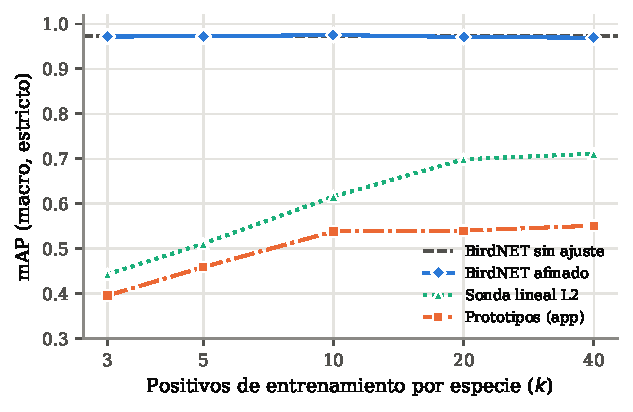
\includegraphics[width=0.68\linewidth]{fig_learning_curve.pdf}\\[6pt]
  {\small\fittab{tab_learning_curve.tex}}
  \caption{mAP estricta en función del número máximo de positivos de entrenamiento por especie.}\label{fig:lc}
\end{figure}

\subsection{Ajuste fino de BirdNET: ablación}
La tabla~\ref{tab:ablation} muestra que reducir $\lambda$ empeora monótonamente la mAP: alejarse de los pesos de BirdNET no ayuda con estas
etiquetas. Con $\lambda = 0{,}3$, la mejor época por pliegue está entre 0 y 6 de 120 posibles
(0 equivale a BirdNET sin cambios): el ajuste se detiene casi de inmediato. Ignorar los pares inciertos en la pérdida (en lugar de
tratarlos como negativos) apenas cambia el resultado, porque son solo 79 pares.

\begin{table}[H]
  \centering\small
  \caption{Variantes del ajuste fino y ablación de los pares inciertos (régimen estricto).}\label{tab:ablation}
  \fittab{tab_ablation.tex}
\end{table}

\subsection{Estructura del espacio de \emph{embeddings}}
La proyección t-SNE \citep{vandermaaten2008tsne} de la figura~\ref{fig:tsne} muestra que la mayoría de especies forman grupos compactos y
separados del fondo, lo que explica el buen rendimiento de clasificadores simples sobre el \emph{embedding}. Algunas especies, como
\spp{Zenaida meloda}, se dividen en varios grupos correspondientes a distintos tipos de vocalización. Este es el motivo de usar varios
prototipos por especie. \spp{Mimus longicaudatus}, con un repertorio muy variable, aparece disperso y cerca del fondo.

\begin{figure}[H]
  \centering
  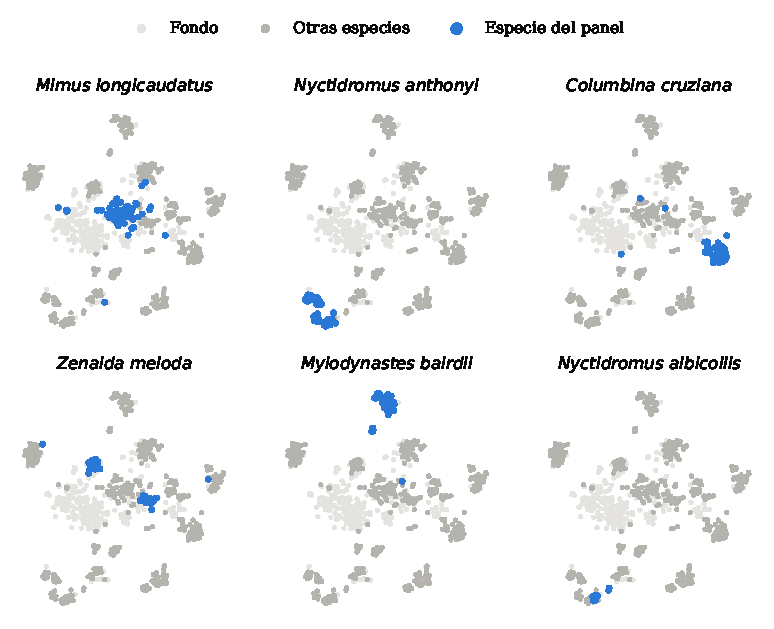
\includegraphics[width=0.95\linewidth]{fig_embedding_tsne.pdf}
  \caption{Proyección t-SNE de \emph{embeddings} BirdNET (ventanas con una sola especie y fondo). Cada panel resalta una especie.}\label{fig:tsne}
\end{figure}

\subsection{Protocolo de revisión y umbrales por especie}\label{sec:umbrales}
Al calcular la fracción validada de las detecciones de BirdNET por umbral (figura~\ref{fig:review}), la mediana entre especies es
\reviewMedianQuarter{} para puntuaciones $\geq 0{,}25$ y cae por debajo de ese umbral. Esto indica que el equipo revisó las detecciones a partir
de una confianza de 0,25 y que casi todas resultaron correctas. Hay dos excepciones claras (tabla~\ref{tab:review}):
\begin{itemize}
  \item \spp{Mimus longicaudatus}: solo el 56\,\% de sus detecciones $\geq 0{,}25$ en el subconjunto figura en TablaFinal, aunque se revisaron
        5\,419 y solo una se rechazó. Lo más probable es que se revisara una muestra limitada por ser la especie más abundante. Así, las detecciones
        no listadas quedan \emph{sin revisar}, no rechazadas.
  \item \spp{Leptotila verreauxi}: un 75\,\% de cobertura, con 3 rechazos de 70.
\end{itemize}
Este hallazgo invalidó la primera regla de umbrales, que calculaba la precisión de BirdNET en el subconjunto contando las detecciones no
listadas como falsas. Con ella, \spp{M.\ longicaudatus} recibía un umbral de 0,95 y una exhaustividad del 9\,\%.

La regla final sigue a \citet{wood2024guidelines}: para cada especie se ajusta una regresión logística de la validez sobre $\operatorname{logit}(p)$ usando
\emph{solo las detecciones revisadas} de TablaFinal (todas las grabaciones, sin la sesión excluida). El umbral es el menor $p$ con
$\Pr(\text{correcta}) \geq 0{,}9$, nunca inferior al umbral de revisión (0,25), porque por debajo no hay evidencia. Para especies sin rechazos
registrados se usa directamente 0,25. El resultado es 0,25 para 30 especies, 0,29--0,34 para \spp{Camptostoma obsoletum} y \spp{Dives warczewiczi},
y 0,5 (valor por defecto) para \spp{Saltator striatipectus}, cuya regresión no alcanza el 90\,\% en ningún punto.

\begin{figure}[H]
  \centering
  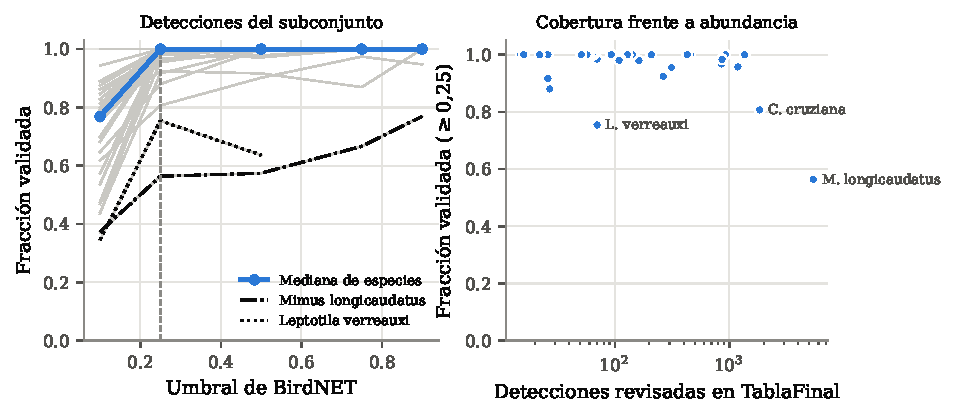
\includegraphics[width=0.95\linewidth]{fig_review_coverage.pdf}
  \caption{Izquierda: fracción de detecciones de BirdNET (recalculadas en el subconjunto) que figuran como validadas, por umbral. Cada línea gris es una especie.
  Derecha: cobertura a 0,25 frente al número de detecciones revisadas en TablaFinal; la especie más abundante es la de menor cobertura.}\label{fig:review}
\end{figure}

\begin{table}[H]
  \centering\small
  \caption{Especies con menor fracción validada de las detecciones de BirdNET (subconjunto) y su revisión en TablaFinal.}\label{tab:review}
  \fittab{tab_review.tex}
\end{table}

\subsection{Detecciones de especies no locales}
Sin filtro geográfico, BirdNET asigna parte de las vocalizaciones a especies de otros continentes, casi siempre congéneres de especies locales
(tablas~\ref{tab:nonlocal} y~\ref{tab:nonlocaltop}). Con umbral 0,5, el \nonlocalHalf\,\% de las detecciones corresponde a especies que no aparecen
entre las 88 validadas de la campaña. Con 0,25 la proporción sube al \nonlocalQuarter\,\%. Restringir la salida a la lista local elimina estos falsos positivos
sin coste para las especies objetivo.

\begin{table}[H]
  \centering\small
  \begin{minipage}[t]{0.42\linewidth}\centering
    \caption{Detecciones de BirdNET (sin filtro geográfico) en el subconjunto.}\label{tab:nonlocal}
    \fittab{tab_nonlocal.tex}
  \end{minipage}\hfill
  \begin{minipage}[t]{0.55\linewidth}\centering
    \caption{Especies no locales más detectadas (puntuación $\geq 0{,}5$).}\label{tab:nonlocaltop}
    \fittab{tab_nonlocal_top.tex}
  \end{minipage}
\end{table}

% ============================================================================
\section{Discusión}\label{sec:discusion}
% ============================================================================
\subsection{¿Por qué el ajuste fino no supera a BirdNET?}
Todas las etiquetas positivas proceden de detecciones de BirdNET con confianza $\gtrsim 0{,}25$ que un experto confirmó. Un canto que BirdNET puntuó
bajo nunca se revisó y cuenta como negativo, aunque sea real. En consecuencia, la etiqueta es casi una función de la puntuación de BirdNET: BirdNET
ordena casi perfectamente sus propias propuestas, y cualquier modelo que discrepe de él pierde AP aunque esté detectando cantos reales. Es el sesgo de verificación
descrito en la sección~\ref{sec:sesgo}. Se aprecia directamente en la figura~\ref{fig:scores}: no hay positivos por debajo de 0,25. Por eso:
\begin{itemize}
  \item la mAP de BirdNET (\mapBirdnet) es una cota optimista de su rendimiento real en este bosque;
  \item el ajuste fino óptimo, según estas etiquetas, es no moverse de BirdNET, y eso es lo que eligen la parada temprana y L2-SP;
  \item comparar con BirdNET no permite saber si un modelo afinado sería mejor detectando lo que BirdNET \emph{no} ve.
\end{itemize}
Medir esa mejora requiere un conjunto de prueba \emph{anotado exhaustivamente}: ventanas elegidas al azar, independientemente de BirdNET, donde el experto
marque todas las especies audibles (sección~\ref{sec:ayuda}).

\subsection{Qué sí muestran los datos}
\begin{enumerate}
  \item \textbf{La biblioteca de perfiles actual es mejorable.} Con los mismos \emph{embeddings}, una cabeza lineal entrenada con positivos y negativos mejora
        la mAP en \deltaLinearVsProto{} sobre los prototipos, con un intervalo de confianza lejos de cero, y generaliza mejor a grabadoras nuevas. Esta comparación no está
        sesgada a favor de ninguno de los dos, porque ambos usan la misma información.
  \item \textbf{BirdNET necesita una lista local.} Entre el 12\,\% y el 23\,\% de sus detecciones, según el umbral, son especies ausentes de la región.
  \item \textbf{Un único umbral no sirve para todas las especies.} La calibración por especie con las validaciones permite fijar umbrales con una precisión
        esperada conocida, como recomiendan \citet{wood2024guidelines}.
  \item \textbf{La revisión por muestreo debe registrarse.} Cuando no se revisan todas las detecciones de una especie, hay que guardar qué se revisó; si no,
        las detecciones no revisadas se confunden con rechazos y sesgan cualquier calibración.
\end{enumerate}

\subsection{Limitaciones}
\begin{itemize}
  \item Se analizó un subconjunto de 257 de las más de 4\,000 grabaciones con detecciones, elegido para cubrir especies, no al azar. Las métricas por especie con pocos
        positivos (p.\,ej.\ \spp{Buteogallus meridionalis}, $n = 11$) tienen alta varianza.
  \item La campaña cubre dos semanas de una estación en una región. La generalización a otras épocas (cambios de actividad vocal) no está evaluada.
  \item Solo se afinó la última capa de BirdNET. Afinar capas convolucionales requeriría el modelo entrenable (no el TFLite) y más datos.
  \item Los negativos implícitos incluyen cantos reales no detectados por BirdNET, lo que penaliza de forma desconocida a todos los métodos distintos de BirdNET.
\end{itemize}

% ============================================================================
\section{Integración en la aplicación}
% ============================================================================
\subsection{Clasificador local CONDESAN}
El módulo \code{local_classifier.py} implementa \code{LocalSpeciesClassifier}:
\begin{itemize}
  \item carga \code{local_models/condesan/condesan_local.json} (especies, nombres, etiquetas BirdNET, umbrales y metadatos);
  \item obtiene los pesos de \code{condesan_local.npz} si el modelo exportado es uno afinado, o, en el caso actual, extrae las 33 columnas
        correspondientes de la capa \code{CLASS_DENSE_LAYER} del BirdNET instalado con la aplicación;
  \item calcula $p = \sigma(W_S^\top \mathbf{e} + \mathbf{b}_S)$ para cada ventana a partir del \emph{embedding} crudo, y emite una detección cuando
        $p$ supera el umbral calibrado de la especie (con un factor de escala opcional).
\end{itemize}
Las detecciones llevan el nombre común en español y la fuente \code{local}. Se muestran en la tabla de resultados con un color propio y se
exportan con el resto.

Se verificó la integración en dos niveles. Primero, sobre 500 ventanas las probabilidades del clasificador coinciden con las de BirdNET para
las mismas especies (diferencia máxima $10^{-4}$, debida al almacenamiento de los logits en media precisión). Segundo, se ejecutó el analizador de la
aplicación (\code{AudioAnalyzer.analyze}) sobre una grabación de AM005 (25/07/2025, amanecer). Produjo exactamente las dos detecciones validadas
en TablaFinal: \spp{Icterus mesomelas} en 42--45\,s y 51--54\,s, con confianzas 0,687 y 0,421 frente a 0,688 y 0,421. Las pruebas unitarias
(\code{tests/test_local_classifier.py}) cubren la carga del modelo, la aplicación de umbrales por especie y la calibración de umbrales.

\subsection{Cambios en la aplicación}
\begin{itemize}
  \item \code{audio_analyzer.py}: nuevo parámetro \code{use_local_classifier} (falso por defecto). Cuando está activo, el analizador extrae los \emph{embeddings}
        crudos de BirdNET (una sola vez, compartidos con los perfiles propios) y suma las detecciones locales a las de los perfiles. Con la opción
        desactivada, el flujo es idéntico al anterior.
  \item \code{main.py}: casilla \emph{Usar clasificador local CONDESAN (BirdNET calibrado)} en el paso de parámetros. Se deshabilita si el modelo no está
        presente, se guarda en la configuración y se registra en el log.
  \item \code{build_exe.py}: incluye la carpeta \code{local_models} en el ejecutable. Se eligió ese nombre, y no \code{models/}, porque el script ya
        interpreta \code{models/} como la carpeta de pesos de BirdNET.
\end{itemize}

\subsection{Recomendaciones de uso}
Para grabaciones del bosque seco de la campaña CONDESAN, se recomienda activar el clasificador local, que reemplaza la lista global por la local con umbrales
calibrados. Las anomalías de BirdNET siguen disponibles para descubrir especies fuera de la lista. Los perfiles manuales con pocos clips (3--5) siguen siendo útiles
para especies nuevas, pero con más de 10 ejemplos conviene entrenar una cabeza lineal (\code{python -m finetuning.train}).

% ============================================================================
\section{Trabajo futuro}
% ============================================================================
\begin{enumerate}
  \item Anotar exhaustivamente un conjunto de prueba aleatorio (p.\,ej.\ 300 ventanas de 3\,s estratificadas por grabadora y periodo) para medir sin sesgo
        el rendimiento de BirdNET y de los modelos afinados.
  \item Ejecutar el pipeline sobre todas las grabaciones (no solo el subconjunto) con la carpeta de Drive sincronizada localmente
        (\code{ECO_DATA_ROOT}).
  \item Sustituir los prototipos de la biblioteca de perfiles por una sonda lineal entrenada con los clips del usuario y negativos de fondo,
        con umbral calibrado por perfil.
  \item Revisar activamente las ventanas donde BirdNET y la sonda discrepan más (aprendizaje activo), que es donde más informa la anotación experta.
  \item Incorporar la semana del año y la hora (amanecer/atardecer) como información previa por especie.
\end{enumerate}

% ============================================================================
\section{Ayuda manual requerida}\label{sec:ayuda}
% ============================================================================
\begin{enumerate}
  \item \textbf{Sesión \code{AM001/20250804/Audio_Sunrise}}: verificar en Drive si los audios corresponden a esa grabadora y fecha. Sus detecciones no coinciden
        con el audio (concordancia \qcExcludedAgreement\,\%).
  \item \textbf{Archivos ausentes de AM003}: \code{20250724_170900}, \code{20250725_073800}, \code{20250726_064100}, \code{20250726_073900},
        \code{20250726_074300}, \code{20250727_070200}, \code{20250727_070300}, \code{20250727_070400} y \code{20250727_073100} figuran en TablaFinal pero no
        en la carpeta de Drive.
  \item \textbf{Protocolo de validación}: confirmar (a) el umbral de confianza usado para generar las detecciones revisadas (los datos sugieren 0,25);
        (b) si las detecciones rechazadas se eliminaron de TablaFinal o se conservaron con \code{Valid}=0, dado que hay solo 79 rechazos;
        y (c) si se revisó una muestra limitada de \spp{Mimus longicaudatus}, \spp{Leptotila verreauxi} u otras especies abundantes.
  \item \textbf{Conjunto de prueba sin sesgo}: anotar todas las especies audibles en la muestra aleatoria de ventanas que genera el notebook de Colab
        (\code{anotacion.xlsx} y un clip de 5\,s por ventana; apéndice~\ref{app:repro}).
  \item \textbf{Datos completos}: para usar todas las grabaciones, ejecutar el pipeline en un equipo con Google Drive para escritorio, o habilitar el acceso
        de red a Google Drive en el entorno de ejecución.
  \item \textbf{Publicación}: el repositorio es público. Solo contiene métricas agregadas, figuras y el modelo de umbrales (ni audio, ni TablaFinal, ni
        detecciones individuales, ni pesos de BirdNET). Confirmar que esto es aceptable para CONDESAN.
\end{enumerate}

\bibliographystyle{plainnat}
\bibliography{referencias}

\appendix
% ============================================================================
\section{Resultados por especie}\label{app:species}
% ============================================================================
\input{\tabdir/tab_species.tex}

% ============================================================================
\section{Reproducibilidad}\label{app:repro}
% ============================================================================
Requisitos: Python 3.11, \code{birdnet-analyzer} 2.4.0 (o un intérprete TFLite) y el modelo BirdNET V2.4 FP32. Variables de entorno:
\code{ECO_DATA_ROOT} (copia local de la carpeta de Drive), \code{ECO_WORK_DIR} (artefactos intermedios) y \code{ECO_BIRDNET_MODEL_DIR}
(carpeta con el \code{.tflite} y las etiquetas).
\begin{lstlisting}
python -m finetuning.select_subset --budget 250 --quota 40   # opcional
python -m finetuning.drive_mirror index                      # indexa los WAV locales
python -m finetuning.embeddings                              # embeddings y logits BirdNET
python -m finetuning.train                                   # CV, LODO, bootstrap, exportacion
python -m finetuning.report                                  # figuras y tablas
python -m finetuning.sample_annotation --n 300 --out ANOTACION  # hoja aleatoria
python -m finetuning.evaluate_annotations --anotacion ANOTACION/anotacion.xlsx
cd docs/informe_finetuning && latexmk -pdf informe_finetuning.tex
\end{lstlisting}
Para el conjunto completo se recomienda Google Colab (CPU, Python 3.13): el notebook \code{finetuning/colab_pipeline.ipynb} lee la carpeta de
Drive sin descargarla, escribe solo en una carpeta nueva (\code{EcoRadar_trabajo}) y retoma la extracción de \emph{embeddings} si la sesión se
interrumpe. La GPU no aporta nada, porque BirdNET TFLite y las cabezas de clasificación corren en CPU.

La muestra para anotar se elige al azar, sin consultar BirdNET, estratificada por grabadora y periodo y alineada con la rejilla de 3\,s de BirdNET.
La evaluación usa las predicciones fuera de muestra de la validación cruzada, de modo que ningún modelo se entrena con la sesión de la ventana que
puntúa, y la anotación nunca se usa para entrenar. Además de la AP de cada método, informa qué fracción de las presencias reales recoge
TablaFinal: es la medida directa del sesgo de verificación.
Artefactos versionados: \code{finetuning/results/} (métricas agregadas, figuras y tablas) y \code{local_models/condesan/condesan_local.json}.
Artefactos no versionados: \code{data_cache/} (audio, TablaFinal, \emph{embeddings}, predicciones fuera de muestra).

\end{document}
